\subsubsection{Matriu de confusió i mètriques de classificació}

Per complementar l’anàlisi individual dels escenaris, s’ha utilitzat una matriu de confusió amb l’objectiu d’avaluar la capacitat del sistema per diferenciar entre operacions potencialment perilloses i operacions que no requereixen una alerta de seguretat elevada.

Per construir aquesta matriu, els nivells de risc proporcionats pel sistema s’han agrupat en dues classes. Una predicció es considera positiva quan el veredicte final és \texttt{MEDIO} o \texttt{ALTO}, o quan l’acció recomanada és revisar l’operació abans de confirmar-la. En canvi, una predicció es considera negativa quan el resultat és \texttt{BAJO} i l’acció recomanada permet continuar sense una alerta elevada.

La classe real de cada prova s’ha definit prèviament a partir de la naturalesa de l’operació executada dins de l’entorn controlat. Es consideren casos positius les aprovacions ERC20 il·limitades, els permisos globals NFT actius i les interaccions amb adreces etiquetades com a malicioses o d’alt risc. Es consideren casos negatius les revocacions de permisos, les aprovacions limitades dirigides als contractes de prova i les transferències simples sense indicadors addicionals de risc.

Aquesta simplificació binària permet calcular els quatre resultats habituals d’una matriu de confusió:

\begin{itemize}
    \item \textbf{Vertader positiu (VP):} una operació realment perillosa és classificada pel sistema com a operació de risc.
    \item \textbf{Fals positiu (FP):} una operació considerada segura dins de l’escenari controlat és classificada com a operació de risc.
    \item \textbf{Vertader negatiu (VN):} una operació segura és classificada correctament com a risc baix.
    \item \textbf{Fals negatiu (FN):} una operació realment perillosa és classificada incorrectament com a risc baix.
\end{itemize}

La Taula~\ref{tab:casos_matriu_confusio} mostra els casos utilitzats per construir la matriu. Cada fila es va executar deu vegades i cada repetició es comptabilitza com una observació independent. La columna \textbf{Classe real} no representa la resposta produïda pel sistema, sinó l'etiqueta de referència assignada abans de la prova segons l'efecte conegut de l'operació. La classe real és \textbf{positiva} quan l'operació hauria de provocar una alerta perquè concedeix un permís crític o implica una adreça de risc; és \textbf{negativa} quan correspon a una operació limitada, una revocació o una transferència sense indicadors de perill. Aquesta etiqueta de referència es compara amb la predicció del prototip per determinar si el resultat és un VP, un VN, un FP o un FN.

\begin{table}[htbp]
\centering
\small
\renewcommand{\arraystretch}{1.2}
\begin{tabularx}{\textwidth}{
    p{0.10\textwidth}
    X
    p{0.18\textwidth}
    p{0.18\textwidth}
    p{0.14\textwidth}
}
\hline
\textbf{Cas} &
\textbf{Operació analitzada} &
\textbf{Classe real} &
\textbf{Predicció del sistema} &
\textbf{Resultat} \\
\hline

A1 &
Transacció simple sense indicadors de risc &
Negativa &
\texttt{BAJO} &
VN \\

B1 &
Aprovació ERC20 limitada a un contracte de prova &
Negativa &
\texttt{BAJO} &
VN \\

B2 &
Revocació ERC20 mitjançant \texttt{approve(spender, 0)} &
Negativa &
\texttt{BAJO} &
VN \\

C1 &
Aprovació ERC20 il·limitada mitjançant \texttt{MaxUint256} &
Positiva &
\texttt{ALTO} &
VP \\

C2 &
Aprovacions ERC20 de frontera amb deu quantitats variables &
7 positives / 3 negatives &
\texttt{BAJO} &
7 FN / 3 VN \\

D1 &
Activació d’un permís global mitjançant \texttt{setApprovalForAll}\allowbreak\texttt{(operator, true)} &
Positiva &
\texttt{ALTO} &
VP \\

D2 &
Revocació del permís global mitjançant \texttt{setApprovalForAll}\allowbreak\texttt{(operator, false)} &
Negativa &
\texttt{BAJO} &
VN \\

E1 &
Interacció amb una adreça etiquetada com a maliciosa o d’alt risc &
Positiva &
\texttt{ALTO} &
VP \\

G1 &
Transacció real limitada sobre Sepolia &
Negativa &
\texttt{BAJO} &
VN (integració) \\

\hline
\end{tabularx}
\caption{Classificació dels casos utilitzats per construir la matriu de confusió}
\label{tab:casos_matriu_confusio}
\end{table}

A partir dels resultats individuals, s’obté la matriu de confusió representada a la Figura~\ref{fig:matriu_confusio}. La intensitat del color de cada cel·la és proporcional al nombre d’observacions que conté, de manera que la concentració dels encerts a la diagonal principal i l’absència de falsos positius resulten immediatament visibles.

\begin{figure}[htbp]
\centering
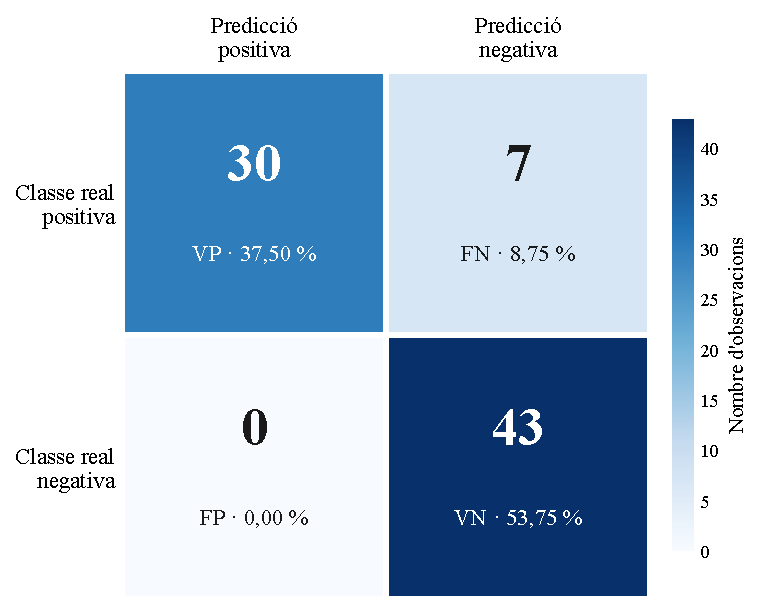
\includegraphics[width=0.78\textwidth]{imgs/matriu_confusio.pdf}
\caption{Matriu de confusió de la classificació de risc}
\label{fig:matriu_confusio}
\end{figure}

A partir de la matriu es poden calcular diverses mètriques quantitatives. L’exactitud representa la proporció total de classificacions correctes:

\[
\text{Exactitud} =
\frac{VP + VN}{VP + VN + FP + FN}
\]

La precisió indica quina proporció de les operacions marcades com a risc eren realment positives:

\[
\text{Precisió} =
\frac{VP}{VP + FP}
\]

La sensibilitat o \textit{recall} mesura la capacitat del sistema per detectar les operacions realment perilloses:

\[
\text{Sensibilitat} =
\frac{VP}{VP + FN}
\]

L’especificitat mesura la capacitat de classificar correctament les operacions segures:

\[
\text{Especificitat} =
\frac{VN}{VN + FP}
\]

Finalment, la mètrica F1 combina la precisió i la sensibilitat en un únic valor:

\[
F1 =
2 \cdot
\frac{\text{Precisió} \cdot \text{Sensibilitat}}
{\text{Precisió} + \text{Sensibilitat}}
\]

Els resultats finals obtinguts són els següents:

\begin{table}[htbp]
\centering
\renewcommand{\arraystretch}{1.25}
\begin{tabular}{l|c}
\hline
\textbf{Mètrica} & \textbf{Resultat} \\
\hline
Exactitud & 0,9125 (91,25\,\%) \\
Precisió & 1,0000 (100\,\%) \\
Sensibilitat & 0,8108 (81,08\,\%) \\
Especificitat & 1,0000 (100\,\%) \\
F1 & 0,8955 (89,55\,\%) \\
\hline
\end{tabular}
\caption{Mètriques obtingudes a partir de la matriu de confusió}
\label{tab:metriques_classificacio}
\end{table}

La matriu es calcula sobre vuit casos i un total de 80 observacions: 37 positives i 43 negatives. El cas C2 aporta set falsos negatius reals: el descodificador només marca com a il·limitada una aprovació exactament igual a \texttt{MaxUint256}, de manera que quantitats lleugerament inferiors, però encara superiors a \(2^{255}\), conserven un veredicte \texttt{BAJO}. Les tres quantitats acotades del mateix cas es classifiquen correctament. G1 valida la integració real i no es torna a comptabilitzar perquè reprodueix una aprovació limitada ja representada per B1.

El resultat mostra que el motor és precís quan genera una alerta, ja que no produeix falsos positius en aquest conjunt, però també identifica una àrea concreta de millora en la sensibilitat davant d'aprovacions extraordinàriament elevades que no coincideixen exactament amb el màxim representable.
